\chapter{Evidence of pair localization in dynamics of Rydberg spins}
\section{Anisotropy-dependent dynamics}
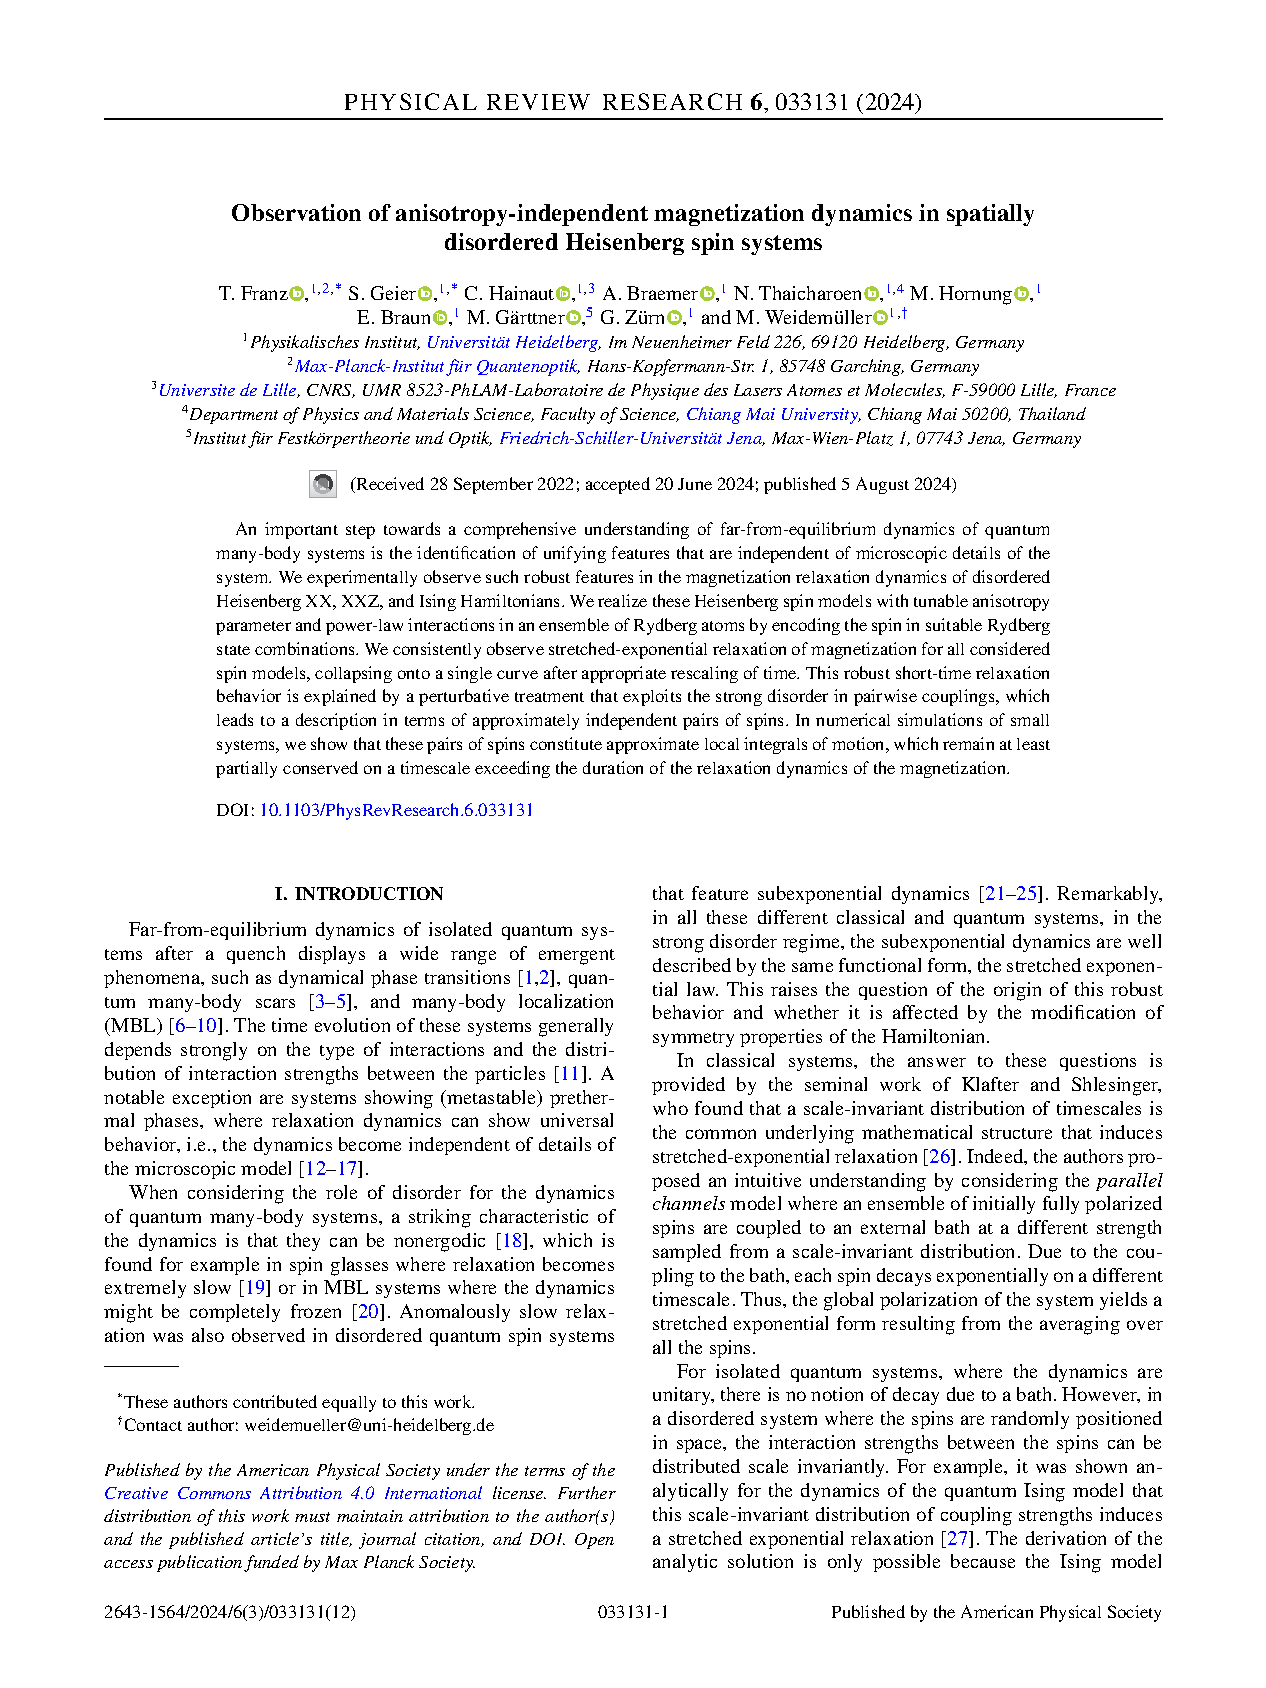
\includepdf[pages=-]{pub-Franz2023-UniversalDynamics}

\section{Emergent pair localization}



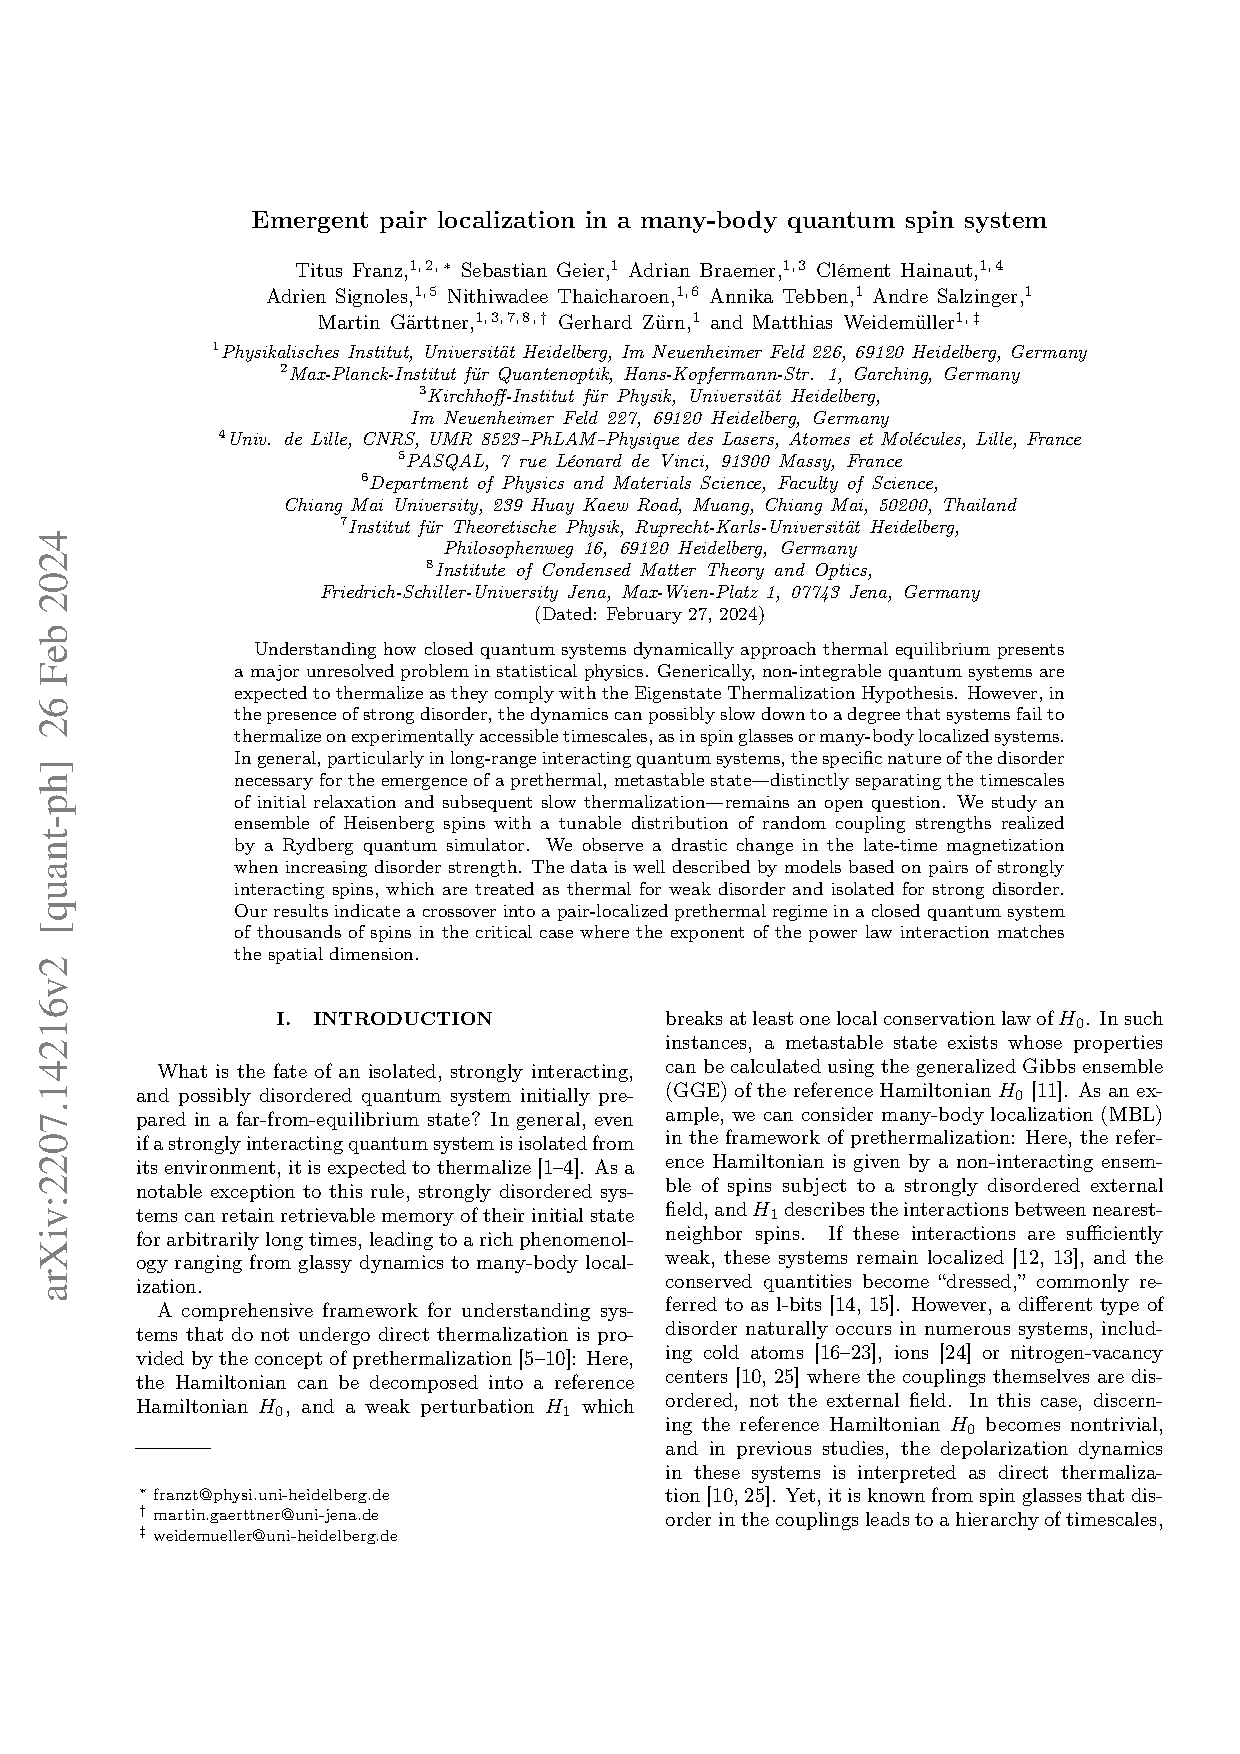
\includepdf[pages=-]{pub-Franz2022-Cusp}

\subsection{Simple physical picture}
\texttt{Cusp-round-sharp.jl}

Two-component model: Each Spin either thermalizes/demagnetizes or stays put. Thus Magnetization is proportional to the cumulative distribution function of the relevant couplings among spins.

Derive distribution functions for nearest neighbor and pair coupling distributions, find qualitative agreement.

\cite{chavezUltraslowGrowthNumber2023}

In the strong disorder limit, \ie $r_b\rightarrow 0$, spins are distributed randomly with uniform density $\rho$ in $d$ dimensional space. Fixing some spin, this gives us for the number of spins in spherical shell of size $r$ and width $\mathrm{d}r$
\begin{equation}\label{eq:uniform-spin-distribution}
	w_u(r)\mathrm{d}r = d \rho \Omega_d r^{d-1}\mathrm{d}r = d\lambda (\lambda r)^{d-1}\mathrm{d}r
\end{equation}
where $\Omega_d = \frac{\pi^{d/2}}{\Gamma(n/2+1)}$ is the volume of a $d$-dimensional unit sphere and $\lambda^d = \rho \Omega_d$ is akin to the inverse mean distance between spins. 

\subsubsection{Nearest-neighbor Coupling Distribution $P_{NN}(J)$}

The distribution of the nearest neighbor couplings can be found using a simple ansatz~\cite{chandrasekharStochasticProblemsPhysics1943}. Consider some fixed spin and the density of spin $w(r)$ at distance $r$. Then the probability $P_{NN}(r)$ of finding the nearest neighbor of that fixed spin at distance $r$ should be proportional to both the probability of having a spin in that distance and the probability of having no closer neighbor. This gives us the following integral-equation 
\begin{align}\label{eq:nn-integral-eq}
	P_{NN}(r) = w(r)*\left(1-\int_0^r \mathrm{d}r' P_{NN}(r')\right)
\end{align}
which can be solved straight-forwardly and yields

\begin{equation}\label{eq:nn-distribution}
	P_{NN}(r) = w(r)\exp\left(-\int_0^r \!\mathrm{d}r' w(r')\right)\quad.
\end{equation}

Plugging in the distance distribution for uniform spin density $w_u(r)$ (cf. Eq.~\ref{eq:uniform-spin-distribution}) gives us a so-called Weibull distribution:

\begin{align}\label{eq:weibull-distribution}
	P_{NN}(r) = d \lambda^d r^{d-1} \exp(- \lambda^d r^d)
\end{align}

%\marginline{Eq.~\ref{eq:weibull-distribution} is a so-called Weibull distribution}

Changing variables from distance $r$ to coupling $J=r^{-\alpha}$ yields
%
%\begin{align}
%	r &= J^{-\frac{1}{\alpha}}\\
%	\mathrm{d}r &= \frac{-1}{\alpha}J^{-\frac{1}{\alpha}-1}\mathrm{d}J
%\end{align}
%
%The sign of the Jacobi-Determinant is to be neglect and we obtain:
%
\begin{equation}
	P_{NN}(J) = \beta\lambda^d J^{-\beta-1} \exp\left(-\lambda^d J^{-\beta}\right)
\end{equation}
where $\beta=\frac{d}{\alpha}$.

\subsubsection{Distribution of Pair Couplings $P_{pair}(J)$}
%TODO clear up difference pair <-> NN?
We can derive the distribution of pair lengths in a similar fashion to Eq.~\ref{eq:nn-integral-eq}. The key insight about the difference between a nearest neighbor and the partner of a pair in the RSRG sense is that the two partners of the pair are in some sense each other's partner. In contrast the "nearest neighbor" property does not need to be reflexive. Denoting the pair coupling distribution as $P_{pair}(J)$, we write down the respective integral equation, which is very similar to Eq.~\ref{eq:nn-integral-eq}, except that the second factor gets squared because \emph{both spins} may not be part of a smaller pair:

\begin{align}\label{eq:pair-integral-eq}
	P_{pair}(r) = w(r)*\left(1-\int_0^r \mathrm{d}r' P_{pair}(r')\right)^2
\end{align}

%We can solve this equation rather easily by separation of variables (easy once you know what to do that is...):
%
%\begin{align}
%	w_P(r) = w(r)*\left(1-\int_0^r \mathrm{d}r' w_P(r')\right)^2\\
%	\Leftrightarrow \int_0^R \mathrm{d}r \frac{w_P(r)}{\left(1-\int_0^r \mathrm{d}r' w_P(r')\right)^2} = \int_0^R \mathrm{d}r w(r)\\
%	\Leftrightarrow \frac{1}{1-\int_0^R \mathrm{d}r' w_P(r')} - 1 = \int_0^R \mathrm{d}r w(r)\\
%	\Leftrightarrow \int_0^R \mathrm{d}r' w_P(r') = 1- \frac{1}{1 + \int_0^R \mathrm{d}rw(r)}\\
%	\Leftrightarrow w_P(R) = \frac{w(R)}{\left(1 + \int_0^R \mathrm{d}rw(r)\right)^2}\\
%	\Rightarrow w_P(r) = \frac{d\mathrm{vol}_d(1)r^{d-1}}{\left(1 + \mathrm{vol}_d(1)r^d\right)^2} = \frac{d}{\lambda} \frac{\left(\frac{r}{\lambda}\right)^{d-1}}{\left( 1+\left(\frac{r}{\lambda}\right)^d\right)^2}
%\end{align}

This equation can be solved in the same way as Eq.~\ref{eq:nn-integral-eq} and yields:

\begin{align}\label{eq:pair-distribution}
	P_{pair}(r) = \frac{w(r)}{\left(1+\int_0^r\!\mathrm{d}r' w(r')\right)^2}
\end{align}

\marginline{Eq.~\ref{eq:pair-integral-eq} was derived by a different method for $d=3$ by former Master student Péter Kaposvári in his Master thesis~\cite{peterMasterThesis}.}

Employing the distance distribution for uniform spin density $w_u(r)$ (cf. Eq.~\ref{eq:uniform-spin-distribution}) again gives us the distribution of pair lengths for uniformly distributed spins:

\begin{equation}\label{eq:log-logistic-distribution}
	P_{pair}(r) = \frac{d\lambda^d r^{d-1}}{\left(1 + \lambda^d r^d\right)^2 }
\end{equation}

\marginline{Eq.~\ref{eq:log-logistic-distribution} is called a log-logistic distribution.}

Changing to distance $r$ to coupling $J=r^{-\alpha}$ yields:

\begin{equation}
	w_P(J) = \frac{\beta\lambda^d J^{-\beta-1}}{\left(1+\lambda^{d}J^{-\beta}\right)^2}
\end{equation}

For $J\rightarrow 0$ this gives the limits:

\begin{equation}
	\lim_{J\rightarrow0} w_P(J) = \lim_{J\rightarrow0} \beta\lambda^{-d} J^{\beta-1} =\begin{cases}0 & d>\alpha\\ \beta\lambda^{-d} & d=\alpha\\ \infty & d<\alpha\end{cases}
\end{equation}

The Cusp thus acquires the form:

\begin{equation}
	\int_0^h\! \mathrm{d}J\ w_P(J) = \left. \frac{1}{1+\lambda^{d}J^{-\beta}}\right|_{0}^h = \frac{1}{1+\lambda^{d}h^{-\beta}}
\end{equation}

Note: For $\alpha > d$ this predicted cusp gets ultra sharp as the first derivative diverges at $0$!

\begin{figure}[ht]
	\centering
	%TODO maybe integrate the curves from CUSP paper for better comparison?
	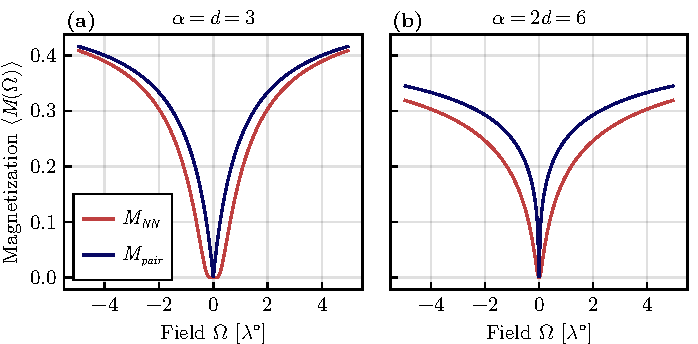
\includegraphics{part1/analytical_cusp}
	\caption{Some sample caption text to compare the size to with a large M}
	\label{fig:analytical-cusp}
\end{figure}